En este capítulo se presentan los resultados y su análisis en relación con las respuestas a las preguntas de investigación planteadas.

%%%%%%%%%%%%%%%%%%%%%%%%%%%%%%%%%%%%%%%%%%%%%%%%%%%%%%%%%%%%%%
\section{Resultados experimentales\label{SEC:TABLAS}}
%%%%%%%%%%%%%%%%%%%%%%%%%%%%%%%%%%%%%%%%%%%%%%%%%%%%%%%%%%%%%%

Las Tablas \ref{TB:RES_PV} a \ref{TB:RES_UTKFULL} muestran las métricas de los seis experimentos, para los conjuntos \textbf{UTKFaceBias}, \textbf{UTKFaceFull} y \textbf{PlantVillage}. El Apéndice \ref{AP:RENDIMIENTO} ofrece información adicional relativa al consumo de recursos y configuración óptima de hiperparámetros para cada experimento.

Se denomina ``\textsc{Clase 0}'' a los hombres en el dataset UTKFace, y a los tomates sanos en PlantVillage. De igual forma, la ``\textsc{Clase 1}'' son las mujeres para UTKFace, y los tomates infectados para PlantVillage. En todos los escenarios de desbalanceo, la ``\textsc{Clase 1}'' es la minoritaria, y la 0 la mayoritaria. Es importante señalar que los experimentos \textbf{WGAN} y \textbf{PRM-IM} no han sido llevados a cabo para el conjunto de datos \textbf{UTKFaceFull}, que presenta un grado de desbalanceo de 1 (sus clases están equilibradas). Esta decisión se debe a que generar muestras minoritarias mediante WGAN, o dividir la clase mayoritaria en conjuntos del mismo tamaño que la clase minoritaria con PRM-IM, carece de sentido en un escenario donde los tamaños de las clases son idénticos, y sus métricas serían equivalentes al experimento \textbf{Baseline}.

\begin{landscape}
\begin{table}[Resultados PlantVillage]{TB:RES_PV}{Resultados para el dataset \textbf{PlantVillage}. En negrita, se resaltan los métodos con las mejores métricas, tanto a nivel de datos como de algoritmo.}
    \small
    % \vskip-0.5cm\begin{tabular}{|c|c|c|c|c|c|c|c|c|c|c|c|}
    \begin{tabular}{|c|c|c|c|c|c|c|c|c|c|c|c|}
    \hline
         &  \multicolumn{4}{c|}{\textsc{Macro average}} & \multicolumn{3}{c|}{\textsc{Clase 0}} & \multicolumn{3}{c|}{\textsc{Clase 1}}\\ \hline
        \textbf{Experimento} & \textbf{Recall} & \textbf{Precisión} & \textbf{F1-score} & \textbf{g-mean} & \textbf{Recall} & \textbf{Precisión} & \textbf{F1-score} & \textbf{Recall} & \textbf{Precisión} & \textbf{F1-score} \\ \hline
        Baseline & 0.9913043 & 0.9913043 & 0.9913043 & 0.9940954 & 0.9968944 & 0.9968944 & 0.9968944 & 0.9857140 & 0.9857140 & 0.9857140 \\ \hline
        WGAN & 0.9985380 & 0.9983766 & \textbf{0.9984549} & \textbf{0.9992687} & 1.0000000 & 0.9967532 & 0.9983740 & 0.9970760 & 1.0000000 & 0.9985359 \\ \hline
        Loss Focal & 0.9984326 & 0.9933333 & 0.9958594 & 0.9976486 & 0.9968652 & 1.0000000 & 0.9984301 & 1.0000000 & 0.9866667 & 0.9932886 \\ \hline
        Loss Focal Difusa & 1.0000000 & 1.0000000 & \textbf{1.0000000} & \textbf{1.0000000} & 1.0000000 & 1.0000000 & 1.0000000 & 1.0000000 & 1.0000000 & 1.0000000 \\ \hline
        PRM-IM & 0.9935642 & 0.9752451 & 0.9845126 & 0.9967769 & 1.0000000 & 0.9501254 & 0.9742123 & 0.9865145 & 1.0000000 & 0.9932542 \\ \hline
        CoSen CNN & 0.9984520 & 0.9929577 & 0.9956787 & 0.9976777 & 0.9969040 & 1.0000000 & 0.9984496 & 1.0000000 & 0.9859155 & 0.9929078 \\ \hline
    \end{tabular}
\end{table}
% \end{landscape}

% \begin{landscape}
\begin{table}[Resultados UTKFaceBias]{TB:RES_UTKBIAS}{Resultados para el dataset \textbf{UTKFaceBias}. En negrita, se resaltan los métodos con las mejores métricas, tanto a nivel de datos como de algoritmo.}
    \small
    % \hskip-1.0cm\begin{tabular}{|c|c|c|c|c|c|c|c|c|c|c|c|}
    \begin{tabular}{|c|c|c|c|c|c|c|c|c|c|c|c|}
    \hline
         &  \multicolumn{4}{c|}{\textsc{Macro average}} & \multicolumn{3}{c|}{\textsc{Clase 0}} & \multicolumn{3}{c|}{\textsc{Clase 1}}\\ \hline
        \textbf{Experimento} & \textbf{Recall} & \textbf{Precisión} & \textbf{F1-score} & \textbf{g-mean} & \textbf{Recall} & \textbf{Precisión} & \textbf{F1-score} & \textbf{Recall} & \textbf{Precisión} & \textbf{F1-score} \\ \hline
        Baseline & 0.6736993 & 0.7705148 & 0.7036496 & 0.8027902 & 0.9566170 & 0.8777644 & 0.9154959 & 0.3907810 & 0.6632650 & 0.4918030 \\ \hline
        WGAN & 0.8830004 & 0.8957965 & \textbf{0.8845087} & \textbf{0.8434530} & 0.8056769 & 0.9495625 & 0.8717222 & 0.9603239 & 0.8420305 & 0.8972953 \\ \hline
        Loss Focal & 0.7457720 & 0.7184976 & 0.7212667 & 0.8043225 & 0.8674699 & 0.9054495 & 0.8860529 & 0.6240741 & 0.5315457 & 0.5741056 \\ \hline
        Loss Focal Difusa & 0.7193296 & 0.7232835 & \textbf{0.7300762} & \textbf{0.8239759} & 0.8985828 & 0.8938326 & 0.8962014 & 0.5400763 & 0.5527344 & 0.5463320 \\ \hline
        PRM-IM & 0.6534153 & 0.7432568 & 0.6253146 & 0.7888770 & 0.9524217 & 0.6132042 & 0.7465416 & 0.3540129 & 0.8725101 & 0.5032451 \\ \hline
        CoSen CNN & 0.5936011 & 0.7620101 & 0.6133879 & 0.7617356 & 0.9774934 & 0.8447749 & 0.9063012 & 0.2097088 & 0.6792453 & 0.3204748 \\ \hline
    \end{tabular}
\end{table}
\end{landscape}

\begin{landscape}
\begin{table}[Resultados UTKFaceFull]{TB:RES_UTKFULL}{Resultados para el dataset \textbf{UTKFaceFull}. En negrita, se resaltan los métodos con las mejores métricas, tanto a nivel de datos como de algoritmo.}
    \small
    % \vskip10.0cm\begin{tabular}{|c|c|c|c|c|c|c|c|c|c|c|c|}
    \begin{tabular}{|c|c|c|c|c|c|c|c|c|c|c|c|}
    \hline
         &  \multicolumn{4}{c|}{\textsc{Macro average}} & \multicolumn{3}{c|}{\textsc{Clase 0}} & \multicolumn{3}{c|}{\textsc{Clase 1}}\\ \hline
        \textbf{Experimento} & \textbf{Recall} & \textbf{Precisión} & \textbf{F1-score} & \textbf{g-mean} & \textbf{Recall} & \textbf{Precisión} & \textbf{F1-score} & \textbf{Recall} & \textbf{Precisión} & \textbf{F1-score} \\ \hline
        Baseline & 0.7561197 & 0.7560004 & 0.7560406 & 0.7552294 & 0.7543403 & 0.74656357 & 0.7504318 & 0.7578991 & 0.7654372 & 0.7616495 \\ \hline
        WGAN & -- & -- & -- & -- & -- & -- & -- & -- & -- & -- \\ \hline
        Loss Focal & 0.7710066 & 0.7702876 & 0.7693955 & 0.7845349 & 0.7983005 & 0.7354759 & 0.7656015 & 0.7437126 & 0.8050994 & 0.7731895 \\ \hline
        Loss Focal Difusa & 0.7878700 & 0.7871188 & \textbf{0.7785564} & \textbf{0.7916486} & 0.7954454 & 0.7545364 & 0.6877871 & 0.7548715 & 0.7045454 & 0.7221489 \\ \hline
        PRM-IM & -- & -- & -- & -- & -- & -- & -- & -- & -- & -- \\ \hline
        CoSen CNN & 0.7253209 & 0.7250534 & 0.7251617 & 0.7205537 & 0.7158177 & 0.7069727 & 0.7113677 & 0.7348243 & 0.7431341 & 0.7389559 \\ \hline
    \end{tabular}
\end{table}
\end{landscape}

En general, los resultados de las tablas revelan la preponderancia en términos de \textit{macro} F1-score y G-mean para los métodos \textbf{WGAN} y \textbf{Loss Focal Difusa}, como se resalta en negrita. Si se presta atención a las métricas desglosadas por clase, se puede ver cómo la presencia de desbalanceo afecta negativamente a la clase minoritaria, y positivamente a la minoritaria. Para encontrar métricas ``equilibradas'' entre las dos clases, hay que dirigirse bien al conjunto \textbf{UTKFaceFull} en la Tabla \ref{TB:RES_UTKFULL} (que tiene la misma proporción de hombres y mujeres); o bien a las métricas de \textbf{WGAN} de las Tablas \ref{TB:RES_PV} y \ref{TB:RES_UTKBIAS}, que representan los escenarios en los que el desbalanceo ha sido mitigado mediante sobremuestreo con imágenes sintéticas.

Las Figuras \ref{FIG:MACROF1} y \ref{FIG:GMEAN} permiten estudiar de manera detallada las métricas \textit{macro} de F1-score y G-mean para los tres datasets. Estos diagramas de barras ayudan a discernir el impacto de las características de cada dataset por separado. En el caso de PlantVillage, compuesto por imágenes muy similares, se observa que las métricas de clasificación superan consistentemente el umbral del 90\%. En contraste, las métricas asociadas a UTKFace, que abarca una amplia variedad de caras humanas en diversos contextos de iluminación, raza y edad, muestran valores más bajos en general. Este contraste destaca la influencia que la similitud y la diversidad entre muestras en los conjuntos de datos pueden tener en el rendimiento de las métricas de clasificación.

\begin{figure}[Macro F1-score]{FIG:MACROF1}{F1-score global para los métodos y datasets.}
    \image{13cm}{}{macrof1}
\end{figure}

\begin{figure}[Macro G-mean]{FIG:GMEAN}{G-mean global para los métodos y datasets.}
    \image{13cm}{}{macrogmean}
\end{figure}

%%%%%%%%%%%%%%%%%%%%%%%%%%%%%%%%%%%%%%%%%%%%%%%%%%%%%%%%%%%%%%
\section{Respuesta a las preguntas de investigación\label{SEC:RESPUESTA_RQS}}
%%%%%%%%%%%%%%%%%%%%%%%%%%%%%%%%%%%%%%%%%%%%%%%%%%%%%%%%%%%%%%

Tanto por medio de la F1-score global (Figura \ref{FIG:MACROF1}) como por la G-mean global (Figura \ref{FIG:GMEAN}), podemos llegar a las mismas conclusiones respecto al rendimiento comparativo de unos métodos y otros en función del escenario de datos y desbalanceo presentes. En este punto, se pueden recordar y responder las dos primeras preguntas de investigación:

\begin{description}
    \item[RQ1:] Para mitigar el sesgo por desbalanceo, ¿es siempre mejor atacar los datos, los algoritmos, o depende de cada situación?
    \item[RQ2:] ¿Es necesario conocer de antemano si el conjunto de datos presenta desbalanceo y, en su caso, el grado de desbalanceo, para determinar el método a aplicar?
\end{description}

%%%%%%%%%%%%%%%%%%%%%%%%%%%%%%%%%%%%%%
% RESPUESTA A RQ1 Y RQ2
%%%%%%%%%%%%%%%%%%%%%%%%%%%%%%%%%%%%%%

La respuesta a la \textbf{RQ1} es que la elección del modelo depende claramente de escenario. En lo que respecta al dataset sencillo, PlantVillage, las métricas de F1-score y G-mean revelan que no hay tanta diferencia entre emplear WGAN frente a la Loss Focal Difusa o la CoSen CNN. Mientras tanto, si nos centramos en UTKFace, comparando los dos escenarios de desbalanceo, podemos ver que el claro ganador es el sobremuestreo por WGAN, seguido de la Loss Focal Difusa, que supera al resto de métodos de mitigación algorítmicos. Las Figuras \ref{FIG:MACROF1} y \ref{FIG:GMEAN} ilustran estas conclusiones.
Por tanto, se puede decir que las características de cada escenario sí determinan el método mitigante a escoger. Si el tiempo de ejecución de los modelos quiere reducirse al mínimo, entonces se recomienda usar un método algorítmico como la Loss Focal Difusa, ya que es el que funciona mejor inmediatamente después de la WGAN para ambos datasets. Como ya se ha mencionado, los métodos algorítmicos no añaden tiempo de ejecución adicional, a diferencia de la mitigación a nivel de datos con WGAN (que requieren un entrenamiento y generación de muestras previo).
En el Apéndice \ref{AP:RENDIMIENTO} se puede observar cómo la WGAN añade hasta 36 horas en tiempo de entrenamiento del generador al del clasificador, que está en el orden de la semana y media.
En cambio, si el tiempo no supone un problema, el sobremuestreo por WGAN es el método más recomendable, ya que no sólo mejora las métricas globales, sino que también equilibra y eleva las métricas de las clases individuales.

En relación a la necesidad de conocer previamente el grado de desbalanceo en relación al método seleccionado (\textbf{RQ2}), se puede observar que en la mayoría de las estrategias algorítmicas (Loss Focal, Loss Focal Difusa y CoSenCNN), no es necesario, ya que los pesos y funciones de pérdida se ajustan de manera adecuada, independientemente del grado de desbalanceo. La única excepción es el método PRM-IM, pues su estrategia de dividir la clase mayoritaria en conjuntos del mismo tamaño que la clase minoritaria no tiene sentido en un escenario donde los tamaños de las clases son idénticos. En cuanto al método de estrategia a nivel de datos (WGAN), sí resulta imprescindible tener conocimiento sobre el desbalanceo del conjunto de datos, dado que ello determina qué hacer (si existe desbalanceo, hay que saber cuántas muestras generar para alcanzar el equilibro de la distribución). Y aún en escenarios de equilibrio de clases, si involucran conjuntos de datos complejos, se puede considerar el realizar un aumento sintético de ambas clases. Aunque el propósito principal no sería mitigar el desbalanceo, se podrían mejorar las métricas de rendimiento al incrementar tanto la densidad de muestras como los atributos presentes.

%%%%%%%%%%%%%%%%%%%%%%%%%%%%%%%%%%%%%%
% RESPUESTA A RQ3
%%%%%%%%%%%%%%%%%%%%%%%%%%%%%%%%%%%%%%

Para terminar con el análsis de resultados, es necesario hacer comparativas entre los resultados obtenidos para el dataset de complejidad menor (PlantVillage) frente al más complejo (UTKFace), y determinar el método mejor en cada caso, dando respuesta a la tercera pregunta de investigación:

\begin{description}    
    \item[RQ3:] ¿Cómo afecta la complejidad del problema a la toma de decisiones sobre el mejor método de mitigación del desbalanceo a aplicar?
\end{description}

Para ello, y de acuerdo a la propuesta de resolución descrita en el \textsc{Capítulo \ref{CAP:METODO}}, se han tomado mediciones estadísticas de distancias de Minkowski, entropía de Shannon y entropía de GLCM para ambos datasets. Las Figuras \ref{FIG:MINKOWSKI} a \ref{FIG:GLCM} muestran histogramas con la distribución de cada una de las tres métricas para cada dataset. Aparte, la Tabla \ref{TB:RESUMEN_VARIANCE} resume estadísticamente las medidas de entropía.

\begin{figure}[Histogramas de distancias de Minkowski]{FIG:MINKOWSKI}{Distancias de Minkowski para el dataset PlantVillage (arriba) y UTKFace (abajo).}
    \centering
    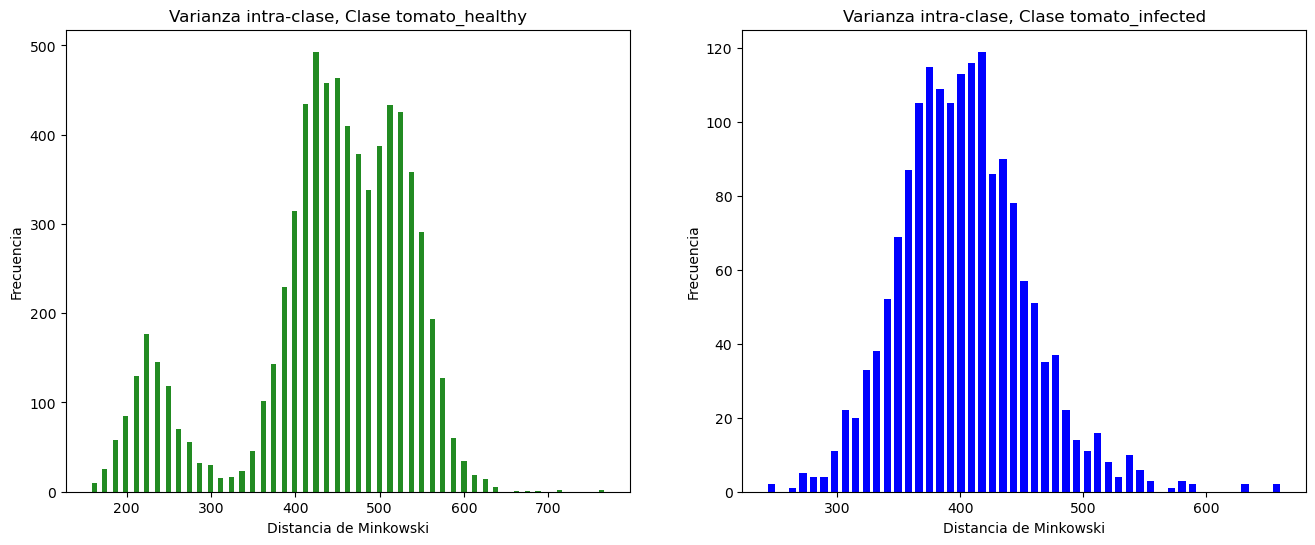
\includegraphics[width=12cm]{img/icv/minkowski_PV.png}
    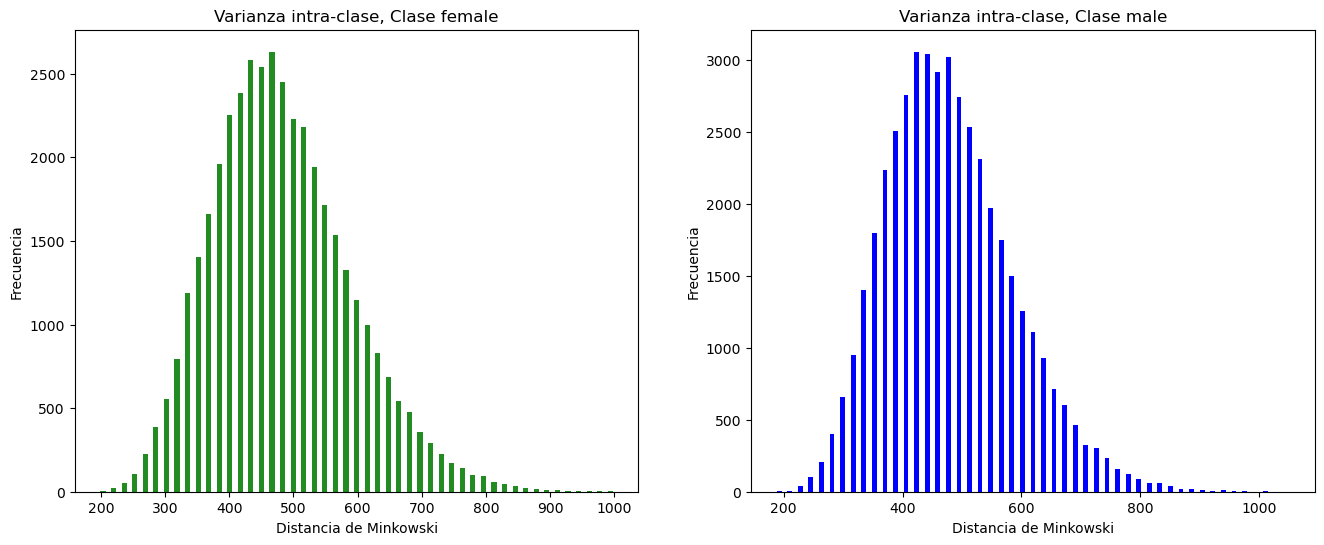
\includegraphics[width=12cm]{img/icv/minkowski_UTK.png}
\end{figure}

\begin{figure}[Entropías de Shannon]{FIG:SHANNON}{Entropías de Shannon para el dataset PlantVillage (izda.) y UTKFace (dcha.).}
    \centering
    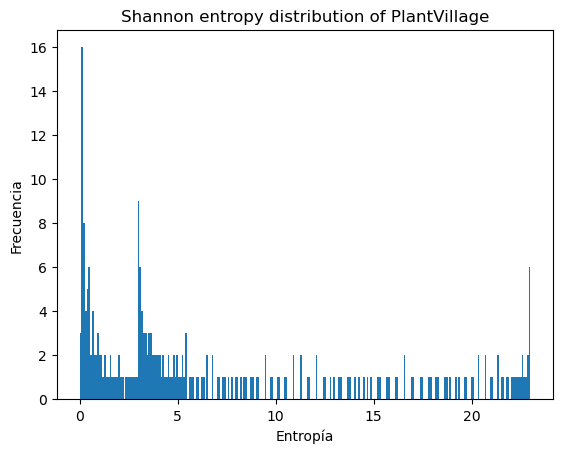
\includegraphics[width=8cm]{img/icv/shannon_PV.png}
    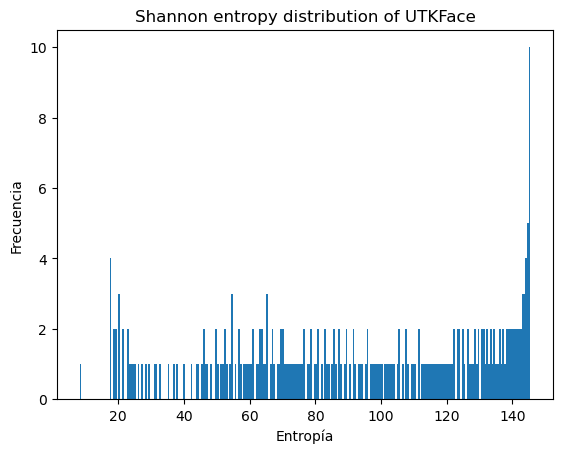
\includegraphics[width=8cm]{img/icv/shannon_UTK.png}
\end{figure}

\begin{figure}[Entropías GLCM]{FIG:GLCM}{Entropías de GLCM para el dataset PlantVillage (izda.) y UTKFace (dcha.).}
    \centering
    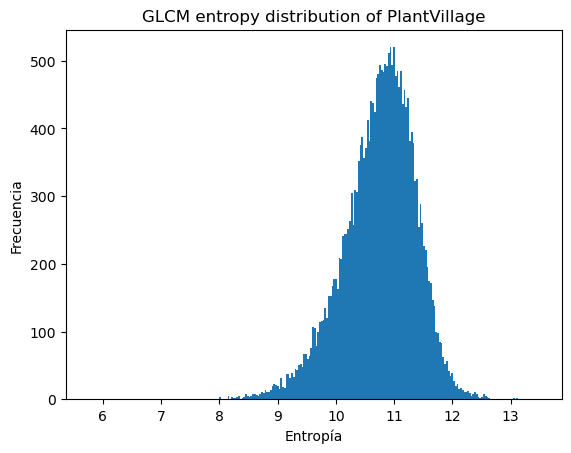
\includegraphics[width=8cm]{img/icv/glcm_PV.png}
    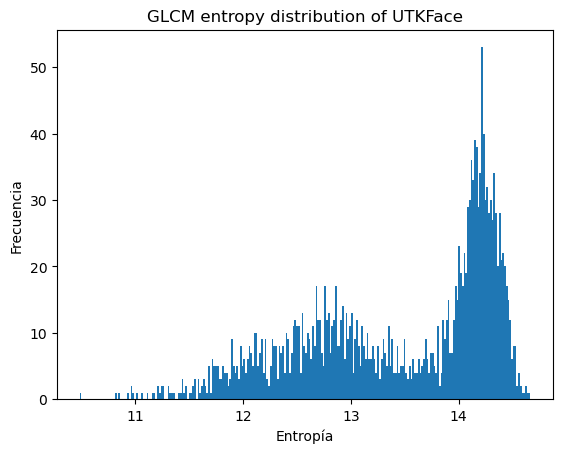
\includegraphics[width=8cm]{img/icv/glcm_UTK.png}
\end{figure}

\begin{table}[Resumen de varianza]{TB:RESUMEN_VARIANCE}{Resumen estadístico de las métricas de entropía para ambos datasets.}
    \small
    \begin{tabular}{|c|c|c|}
    \hline
        \textsc{Dataset} & \textsc{Shannon (media)} & \textsc{GLCM (media/std)} \\ \hline
        PlantVillage & 7.0906 & 13.4438 / 0.8817 \\ \hline
        UTKFace & 7.2627 & 10.7452 / 0.6235 \\ \hline
    \end{tabular}
\end{table}

Las gráficas de la Figura \ref{FIG:MINKOWSKI} son especialmente reveladoras a la hora de hablar de la distribución intra-clase de los conjunto de datos. Aunque para ambos la mayoría de muestras presentan una distancia relativa de entre 400 y 500, es notable cómo en UTKFace hay más \textit{outliers}, para los que la distancia con respecto al resto aumenta a 900 e incluso a 1000. Por su parte, las distancias de Minkowski para PlantVillage siempre están acotadas en un rango reducido que no rebasa los 700.

En cuanto a las métricas de entropía, el histograma de Shannon de PlantVillage (Figura \ref{FIG:SHANNON}) muestra una concentración de bajas entropías, lo cual aventura una alta similaridad entre muestras. Esto es comprensible, ya que se trata de imágenes de plantas de tomate, muy similares entre sí. Por otro lado, el histograma de Shannon de UTKFace muestra una mayor concentración en las entropías altas, lo que indica una alta diversidad entre las instancias de imágenes (imágenes faciales en distintas configuraciones de género, raza, edad y condiciones ambientales). Estas conclusiones son extrapolables a la entropía por GLCM (Figura \ref{FIG:GLCM}), que caracteriza mejor la variabilidad de texturas. El motivo de que en este caso ambos histogramas estén en una escala similar (con entropías entre 10 y 15) puede deberse a que, si bien las imágenes de PlantVillage son muy parecidas entre sí, presentan alta cantidad de grano fotográfico, lo que puede hacer que la caracterización de su textura sea más ``rugosa''. En definitiva, estas métricas permiten cuantificar la noción de ``complejidad'' presente en un dataset de imágenes, en base a dos aspectos fundamentales:

\begin{enumerate}
    \fontsize{11pt}{12pt}\selectfont
    \item Distancia de Minkowski entre imágenes dentro de un rango acotado (más o menos por debajo de 700), lo que implica que 
    % existe una menor variabilidad entre las distancias entre las imágenes. En otras palabras,
    las imágenes exhiben patrones de similitud más marcados en cuanto a las relaciones de proximidad.
    
    \item Una baja entropía, principalmente en términos de la información de Shannon, pero también en la textura caracterizada mediante GLCM. La baja entropía indica una mayor uniformidad y homogeneidad en las características visuales capturadas por las imágenes, y en forma de histograma se caracterizará por un ``pico'' en los valores próximos a cero.
\end{enumerate}

Volviendo a la pregunta \textbf{RQ3}, si la complejidad del dataset es elevada, es mejor idea realizar un aumento de datos con WGAN, siempre y cuando exista una base lo suficientemente grande como para que el generador aprenda a producir muestras aceptables. Ello maximizará las métricas de clasificación. En cambio, para datasets de poca complejidad (como PlantVillage) basta con aplicar un método a algorítmico para paliar el desbalanceo, y seguir logrando métricas elevadas. En este caso, las tablas de resultados y las gráficas parecen indicar que el método propio, la Loss Focal Difusa, es un buen candidato.
Por último, cabe recordar que pueden existir escenarios en los que la aplicación de métodos algorítmicos sea la única vía para mitigar el desbalanceo. Como se señala en \citet{liu2022solving}, a veces la generación sintética de muestras puede ser un error ético, o incluso negligente. Por ejemplo, si la clase minoritaria la componen imágenes de radiografías de pulmones enfermos \cite{rahimzadeh2020modified,narayanan2020transfer}, puede que no sea adecuado aplicar la generación sintética para mitigar el desbalanceo (aun cuando puedan crearse muestras altamente realistas), ya que en ese caso los modelos aprenderían las características de la enfermedad sobre muestras de pacientes que realmente no existen.